\documentclass[10pt, a5paper]{article}
\usepackage{pdfpages}
\usepackage{parallel}
\usepackage[T2A]{fontenc}
\usepackage{ucs}
\usepackage[utf8x]{inputenc}
\usepackage[polish,english,russian]{babel}
\usepackage{hyperref}
\usepackage{rotating}
\usepackage[inner=2cm,top=1.8cm,outer=2cm,bottom=2.3cm,nohead]{geometry}
\usepackage{listings}
\usepackage{graphicx}
\usepackage{wrapfig}
\usepackage{longtable}
\usepackage{indentfirst}
\usepackage{array}
\newcolumntype{P}[1]{>{\raggedright\arraybackslash}p{#1}}
\frenchspacing
\usepackage{fixltx2e} %text sub- and superscripts
\usepackage{icomma} % коскі ў матэматычным рэжыме
\PreloadUnicodePage{4}

\newcommand{\longpage}{\enlargethispage{\baselineskip}}
\newcommand{\shortpage}{\enlargethispage{-\baselineskip}}

\def\switchlang#1{\expandafter\csname switchlang#1\endcsname}
\def\switchlangbe{
\let\saverefname=\refname%
\def\refname{Літаратура}%
\def\figurename{Іл.}%
}
\def\switchlangen{
\let\saverefname=\refname%
\def\refname{References}%
\def\figurename{Fig.}%
}
\def\switchlangru{
\let\saverefname=\refname%
\let\savefigurename=\figurename%
\def\refname{Литература}%
\def\figurename{Рис.}%
}

\hyphenation{admi-ni-stra-tive}
\hyphenation{ex-pe-ri-ence}
\hyphenation{fle-xi-bi-li-ty}
\hyphenation{Py-thon}
\hyphenation{ma-the-ma-ti-cal}
\hyphenation{re-ported}
\hyphenation{imp-le-menta-tions}
\hyphenation{pro-vides}
\hyphenation{en-gi-neering}
\hyphenation{com-pa-ti-bi-li-ty}
\hyphenation{im-pos-sible}
\hyphenation{desk-top}
\hyphenation{elec-tro-nic}
\hyphenation{com-pa-ny}
\hyphenation{de-ve-lop-ment}
\hyphenation{de-ve-loping}
\hyphenation{de-ve-lop}
\hyphenation{da-ta-ba-se}
\hyphenation{plat-forms}
\hyphenation{or-ga-ni-za-tion}
\hyphenation{pro-gramming}
\hyphenation{in-stru-ments}
\hyphenation{Li-nux}
\hyphenation{sour-ce}
\hyphenation{en-vi-ron-ment}
\hyphenation{Te-le-pathy}
\hyphenation{Li-nux-ov-ka}
\hyphenation{Open-BSD}
\hyphenation{Free-BSD}
\hyphenation{men-ti-on-ed}
\hyphenation{app-li-ca-tion}

\def\progref!#1!{\texttt{#1}}
\renewcommand{\arraystretch}{2} %Іначай формулы ў матрыцы зліпаюцца з лініямі
\usepackage{array}

\def\interview #1 (#2), #3, #4, #5\par{

\section[#1, #3, #4]{#1 -- #3, #4}
\def\qname{LVEE}
\def\aname{#1}
\def\q ##1\par{{\noindent \bf \qname: ##1 }\par}
\def\a{{\noindent \bf \aname: } \def\qname{L}\def\aname{#2}}
}

\def\interview* #1 (#2), #3, #4, #5\par{

\section*{#1\\{\small\rm #3, #4. #5}}

\def\qname{LVEE}
\def\aname{#1}
\def\q ##1\par{{\noindent \bf \qname: ##1 }\par}
\def\a{{\noindent \bf \aname: } \def\qname{L}\def\aname{#2}}
}

\begin{document}
\title{Некоммерческая 3D-печать}
\author{Алексей Бабахин, Рязань, РФ\footnote{\url{tamerlan311@mail.ru}, \url{http://lvee.org/ru/abstracts/166}}}
\maketitle
\begin{abstract}
3D printing or additive manufacturing is a process of making three-dimensional solid objects from a digital file. The creation of a 3D printed object is achieved using additive processes, when object is created by laying down successive layers of material one by one until the entire model is recreated. Each of these layers can be seen as a thinly sliced horizontal cross-section of the eventual object.
\end{abstract}
\subsection*{Введение}

Наиболее простой доступной для домашнего применения является технология FDM (метод послойного наплавления). Большим толчком для развития домашней 3D-печати послужили различные стадии открытого проекта RepRap, из которых (или на их базе) сейчас выросло большинство конструкций современных принтеров, представленных на рынке.
Большинство принтеров можно рассматривать как конструктор, включающий три ортогональные подсистемы:

\begin{itemize}
  \item станину принтера --- его механическую часть, которая может различаться очень сильно от модели к модели;
  \item контроллер и его прошивку (controller firmware) --- управляющий блок принтера, который приводит механизм в движение;
  \item слайсер (slicer) --- программу, конвертирующую 3D-модель в послдовательность движений принтера (в G-код)
\end{itemize}

Независимо от того, собран принтер самостоятельно из подручных материалов или это --- купленная <<высокотехнологичная>> заводская модель, которая должна (по заявлению производителя) печатать <<из коробки>>  -- в той или иной степени принтер все равно остаётся конструктором.

\subsection*{Станина}

От типа и жесткости исполнения конструкции сильно зависит качество распечатанных изделий, скорость и ускорение, с которыми сможет печатать принтер.

\subsection*{Контроллер}

Как правило, это модуль, управляемый восьмибитным микроконтроллером, задачей которого является непрерывное управление всеми элементами принтера: 4--5 шаговыми двигателями, 2--3 нагревательными элементами, опционально вентиляторами и графическим экраном. Программу печати контроллер может получать как с flash-карты, так и по кабелю с компьютера (с помощью более-менее специализированного коммуникационнго ПО).

\subsection*{Слайсер}

Программа, которая <<разрезает>> трехмерную модель формата STL или OBJ по слоям и просчитывает все необходимые движения принтера, выдавая на выходе G-код. В зависимости от сложности модели, процесс может требовать значительных вычислительных ресурсов, а также иметь огромное количество настроек. По этой причине слайсинг требует большого количества экспериментов для получения хорошего результата.

\subsection*{Конвейер 3D-печати}

Стадии, которые проходит 3D-модель от ее создания в САПР до печати, представлены на следующей схеме:

\begin{figure}[h!]
  \centering
  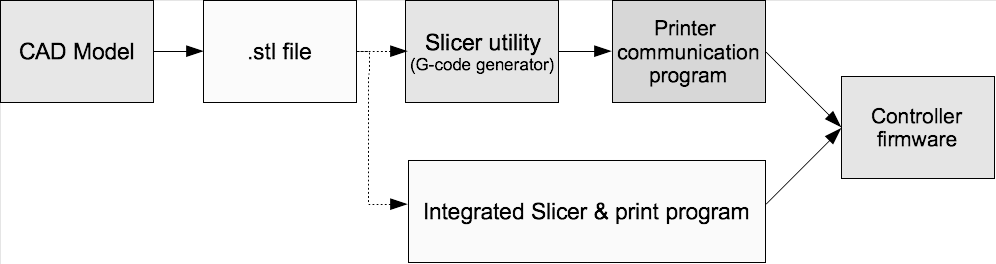
\includegraphics[scale=0.3]{19_2015_fig1}
\end{figure}

Среди популярных слайсеров можно отметить Skeinforge \cite{skeinforge} \linebreak (GPL v.3, изобилие настроек, интерфейс на TCL/TK), его форк skFrontend \cite{sfact}, а также Slic3r \cite{slic3r} (AGPL v.3, поддержка многопоточности, интерфейс на wxWidgets, считается более эргономичным и быстрым, но менее совершенным, чем Skeinforge). В качестве коммуникационного ПО может использоваться Printrun \cite{printrun} (GPL v.3). Кроме того, есть несколько интегрированных решений all-in-one, часто создававшихся для конкретного 3D-принтера, но в последствии ставших достаточно универсальными: cura \cite{cura} (AGPL v.3, частично использует код Skeinforge для слайсинга), RepetierHost \cite{RepetierHost} (лицензия Apache, позволяет выполнять слайсинг с помощью Skeinforge либо Slic3r), Repsnapper \cite{repsnapper} (GPL, в отличие от предыдущих проектов, преимущественно написанных на Python, данный переписан с нуля на С++ и, уступая в настоящий момент в функциональности, взамен обеспечивает наиболее быстрый слайсинг).


\subsection*{Расходные материалы}

Для печати по технологии FDM используются различные пластики в виде круглой нити, намотанной на катушку. Стандартные диаметры --- 3~мм и 1.75~мм. Наиболее популярными являются пластики PLA и ABS. PLA считается самым простым в использовании, т.~к. не требует обязательного горячего стола, печатается при наиболее низкой температуре и не выделяет вредных веществ в процессе печати. Пластик ABS технологичнее (менее хрупкий, не разлагается со временем), но даёт большую усадку при остывании (детали могут деформироваться в процессе печати), а поэтому требует обязательного подогрева платформы, на которой происходит печать. Помимо PLA и ABS также иногда используются менее популярные варианты: Нейлон, Поликарбонат, Полистирол, Полиэтилентерефталат (PET), различные полимерные смеси имитирующие дерево, бронзу и т.~д.

\begin{thebibliography}{9}
\bibitem{skeinforge} \url{http://fabmetheus.crsndoo.com}
\bibitem{sfact} \url{https://github.com/ahmetcemturan/SFACT}
\bibitem{slic3r} \url{http://slic3r.org/}
\bibitem{printrun} \url{https://github.com/kliment/Printrun}
\bibitem{cura} \url{https://github.com/daid/Cura}
\bibitem{RepetierHost} \url{https://github.com/repetier/Repetier-Host}
\bibitem{repsnapper} \url{https://github.com/timschmidt/repsnapper}
\end{thebibliography}

\end{document}
